\documentclass[12pt, a4paper, lithuanian]{article}
\usepackage[utf8x]{inputenc}
\def\LTfontencoding{L7x}
\PrerenderUnicode{ąčęėįšųūž}
\usepackage[\LTfontencoding]{fontenc}
\usepackage[lithuanian]{babel}
\usepackage{VUMIFPSkursinis}
\usepackage{cite}
\usepackage{amsmath}
\usepackage{bm}
\usepackage{amsfonts}
\usepackage{float}
\usepackage{graphicx}
\usepackage{color}
\usepackage{listings}
\usepackage{wrapfig}
\usepackage{algpseudocode}
\usepackage{algorithm}
\usepackage{algorithmicx}
\usepackage{caption}
\usepackage{subfig}


% Titulinio aprašas
\vumifdept{Programų sistemų katedra}
\vumifpaper{Kursinis darbas}
\title{Biojutiklio su selektyvia membrana kompiuterinis modeliavimas}
% \title{Esama situacija su dviem sluoksniais}
% \title{Ištirti selektyvios membranos įtaką amperometrinio bijojutiklio jautriui}
\def\titleineng{Computational modelling of biosensors with selective membranes}
\def\statusas{% Kai kurioms katedroms reikia nurodyti  
    4 kurso 1 grupės studentas \\
}
\author{
   Kęstutis Gimbutas
}

\supervisor{prof. dr. Romas Baronas}
\date{Vilnius – \the\year}

\begin{document}
\sloppy
\maketitle

\tableofcontents

\sectionnonum{Įvadas}
Biojutikliai yra analitiniai prietaisai, kurių pagrindinės sudedamosios dalys
yra biologinis darinys, kuris atpažįsta norimus cheminius junginius, ir
prietaisas, kuris to junginio atpažinimą  paverčia į elektros signalą. Elektros
signalo stiprumas yra proporcingas minėto cheminio elemento koncentracijai
nagrinėjamoje terpėje. Biojutikliai yra klasifikuojamini pagal įrenginio, kuris
paverčia vienos rūšies energiją kita,
prigimtį. Amperometriniai biojutikliai matuoja srovės stiprį faradais, kuri
kyla elektrode dėl biocheminės reakcijos produktų tiesioginės cheminės oksidacijos 
arba redukcijos. Kol matuojama srovė amperometriniuose biojutikliuose elektrodo potencialas yra
laikomas konstanta. Amperometriniai biojutikliai yra žinomi
kaip patikimi, pigūs ir reikšmingi medicinos, pramonės sritims
\cite{baronas2006computational}.

Praktiškas biojutiklis turi daugiasluoksnę fermento membraną. Elekrodas veikia
kaip biojutiklio rėlė, jis yra padengtas selektyviaja membrana po kurios seka
imobilizuotas fermentas. Selektyvioji membrana yra naudojama norint padidinti
biojutiklio selektyvumą \cite{baronas2006computational}. \\

\section{Biojutiklio su selektyvia membrana modelis}
%Sudarant modelius bei lygtis buvo pasinaudota šaltiniais:
%\cite{baronas2009mathematical}, \cite{baronas2006computational},
%\cite{baronas2003influence}.

\subsection{Matematinis modelis}
Remiantis supaprastinta schema tirpalas (S) prisijungia prie fermento (E)
ir yra
paverčiamas į produktą (P),
\begin{equation}\label{eq:basic} 
    S \overset{E}{\rightarrow} P
\end{equation}

Biojutiklio veikimo sistemos lygiai: tirpalas, fermento sluoksnis($\Omega_2$),
selektyvios
membranos sluoksnis($\Omega_1$), elektrodas.

\begin{figure}[H]
    \centering
    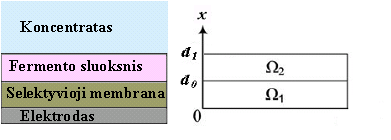
\includegraphics[scale=0.9]{img/modv1}
    \caption{Biosensorio struktūra}
    \label{img:mlp}
\end{figure}

Uždaros sritys atvaizduotos pirmame paveiksle:
\begin{equation}
\begin{aligned}
    &\overline{\Omega}_1 = [0, d_0],\\
    &\overline{\Omega}_2 = [d_0, d_1]
\end{aligned}
\end{equation}

Tegu $\Omega_i$ yra atviros sritys atitinkačios uždarus regionus
$\overline{\Omega}_i$, i = 1, 2:

\begin{equation}
\begin{aligned}
    &\Omega_1 = (0, d_0),\\
    &\Omega_2 = (d_0, d_1)
\end{aligned}
\end{equation}

Regione $\Omega_1$ vyksta tik produkto
difuzija, tuo tarpu $\Omega_2$ regione vyksta fermento
reakcija su substratu ir jų transportavimas taip pat difuzija.

Pagrindinės lygtys ($0<t$):
\begin{equation}
    \frac{\partial P_1}{\partial t} = D_{1P} \frac{\partial^2 P_1}{\partial x^2}, \;
    \; x \in \Omega_1,\;\; t > 0.
\end{equation}

\begin{equation}
\begin{aligned} 
    &\frac{\partial S}{\partial t} = D_S \frac{\partial^2 S}{\partial x^2} -
    \frac{V_{max} S}{K_M + S},  \\ 
    &\frac{\partial P_2}{\partial t} = D_{2P} \frac{\partial^2 P_2}{\partial x^2} +
    \frac{V_{max} S}{K_M + S}, \; \; x \in \Omega_2 ,\;\; t > 0.
\end{aligned}
\end{equation}


\subsection{Pradinės ir kraštinės sąlygos}
\begin{equation}
\begin{aligned}
    &S(0,0) = 0, \\
    &S(x, 0) = 0,\; x \in \Omega_2,\\
    &S(d_1, 0) = S_0,
\end{aligned}
\end{equation}

\begin{equation}
\begin{aligned}
    &P_1(x, 0) = 0,\; x \in \overline\Omega_1,\\
\end{aligned}
\end{equation}

\begin{equation}
\begin{aligned}
    & P_2(x, 0) = 0,\; x \in \Omega_2%,\\
%    &P_2(d_1, 0) = P_0
\end{aligned}
\end{equation}

\begin{equation} 
    P_1(0,t)=0, \; t>0.
\end{equation}

%\begin{equation} 
%    \left. D_S \frac{\partial S}{\partial x} \right|_{x=d_0} = 0, t>0.
%\end{equation}

\begin{equation} 
    S(d_1, t) = S_0,\; t>0,
\end{equation}

\begin{equation} 
    P_2(d_1, t) = 0,\; t>0.
\end{equation}

\begin{equation} 
\begin{aligned}
    \left. \frac{\partial S}{\partial x} \right|_{x=d_0} = 0, \;\;
    & \left. D_{1P} \frac{\partial P_1}{\partial x} \right|_{x=d_0} = 
    \left. D_{2P} \frac{\partial P_2}{\partial x} \right|_{x=d_0},\; t > 0 \\
    & P_1(d_0, t) = P_2(d_0, t),\; t>0.
\end{aligned}
\end{equation}

\subsection{Biojutiklio atsako charakteristikos}
\subsubsection{Atsako laikas}
\begin{equation} 
    i(t) \approx n_eFD_pP/h 
\end{equation}
\begin{equation} 
\begin{aligned}
    T = \underset{i(t)>0}{min}\left\{t:\frac{t}{i(t)} \left| \frac{\partial i(t)}{\partial t}
    \right| < \epsilon \right\}
\end{aligned}
\end{equation}
 
\subsection{Skaitinis lygčių aproksimavimas}
\subsubsection{Neišreikštinė schema}

\begin{equation}
\begin{aligned} 
    &\frac{S_i^{j+1} - S_i^j}{\tau} = D_S\frac{S_{i+1}^{j+1} -
    2S_i^{j+1} + S_{i-1}^{j+1}}{h^2} -
    \frac{V_{max} S_i^j}{K_M + S_i^j},\;i = k,\;...,\;N-1\\ 
    &\frac{P_i^{j+1} - P_i^j}{\tau} = D_{2P}\frac{P_{i+1}^{j+1} -
    2P_i^{j+1} + P_{i-1}^{j+1}}{h^2} +
    \frac{V_{max} S_i^j}{K_M + S_i^j},\;i = k,\;...,\;N-1\\ 
    &\frac{P_i^{j+1} - P_i^j}{\tau} = D_{1P}\frac{P_{i+1}^{j+1} -
    2P_i^{j+1} + P_{i-1}^{j+1}}{h^2}, \;i = 1,\;...,\;k-1\\ 
    &j=0,\;...,\;M-1.
\end{aligned}
\end{equation}

% \subsubsection{Pradinės ir kraštinės modelio sąlygos}
% \begin{equation}
% \begin{aligned}
%     &S_i^0 = 0, i = 0,\;...,\;N-1,\\
%     &S_N^0 = S_0,
% \end{aligned}
% \end{equation}
% 
% \begin{equation}
% \begin{aligned}
%     &P_i^0 = 0, i = 0.\;...,\;N-1,\\
%     &P_N^0 = P_0
% \end{aligned}
% \end{equation}
% 
% \begin{equation} 
%     S_0^j = S_1^j, S_N^j = S_0, j=1,\; ...,\;M, 
% \end{equation}
% 
% \begin{equation} 
%     P_0^j = 0, P_N^j = P_0, j=1,\; ...,\;M, 
% \end{equation}
% 
\subsubsection{Skaičiavimo procedūra}

\begin{equation} 
    i(t_j) \approx t_j = n_eFD_pP_i^j/h,\; j=1,\;...,\;M. 
\end{equation}

\subsection{Skaitinio sprendimo tikrinimas}
% \subsubsection{Pradinės skaičiavimų sąlygos}
% 
% \begin{equation}
% \begin{aligned}
%     &S_0 = 1 \mathrm{\mu M},\; P_0 = 0 \mathrm{\mu M},\\
%     &D_s = 300 \mathrm{\mu m^2/s},\; D_p = 300 \mathrm{\mu m^s/s},\\
%     &T = 50\mathrm{s},\;\; d_0 = *\ \mathrm{\mu m},\; d_1 = *\ \mathrm{\mu m},\;\\
%     &\tau = 0.1\mathrm{s},\; h=0.1 \mathrm{\mu m},\\
%     &V_{max} = 100\mathrm{\mu M /s},\; \epsilon = 0.05,\\
%     &F=961485,\; K_M= 100\mathrm{\mu M},\; n_e = 2.
% \end{aligned}
% \end{equation}
% 
\subsubsection{Gautos matricos iš neišreikštinės schemos}
\textit{Lygčių sistemos gautos naudojant baigtinių skirtumų medodą ir neišreikštines
schemas. Lygtys išsprėstos taikant triįstrižainių matricų algoritmą. Laiko
žingsnis - $\tau$ (indeksas $j$), erdvės žingsnis - $h$ (indeksas $i$).}
\begin{equation}
\left\{
\begin{aligned}
    &S_{i+1}^{j+1}-S_i^{j+1}\left(1+\frac{h^2}{D_S\tau}\right)
= \frac{h^2}{D_S\tau} \left(\frac{V_{max}S_i^j\tau}{K_M+S_i^j}-S_i^j\right),\; \;
i = k +1,\\
    &\dots\;,\\
    &S_{i-1}^{j+1}-S_i^{j+1}\left(2+\frac{h^2}{D_S\tau}\right)+S_{i+1}^{j+1}
        = \frac{h^2}{D_S\tau}
        \left(\frac{V_{max}S_i^j\tau}{K_M+S_i^j}-S_i^j\right),\; \; i =
        k +2,\;...,\;N-1,\\
    &\dots\;,\\
    &S_0 + S_{i-1}^{j+1} - S_i^{j+1}\left(2+\frac{h^2}{D_S\tau}\right)
        =  \frac{h^2}{D_S\tau}
    \left(\frac{V_{max}S_i^j\tau}{K_M+S_i^j}-S_i^j\right),\; \; i = N.
\end{aligned}
\right.
\end{equation}

\begin{equation}
\left\{
\begin{aligned}
%    &P_{i+1}^{j+1}-P_i^{j+1}\left(2+\frac{h^2}{D\tau}\right)
%    = \frac{h^2}{D\tau} \left(-P_i^j -\frac{V_{max}S_i^j\tau}{K_M+S_i^j}\right),\; \; i = 1,\\
    &P_{i+1}^{j+1}-P_i^{j+1}\left(2+\frac{h^2}{D_{1P}\tau}\right)
    = -\frac{h^2}{D_{1P}\tau} P_i^j,\; \; i = 1,\\
    &\dots\;,\\
%    &P_{i-1}^{j+1}-P_i^{j+1}\left(2+\frac{h^2}{D\tau}\right)+P_{i+1}^{j+1}
%        = \frac{h^2}{D\tau}
%    \left(\frac{V_{max}S_i^j\tau}{K_M+S_i^j}-S_i^j\right),\; \; i =
%        2,\;...,\;k-1,\\
    &P_{i-1}^{j+1}-P_i^{j+1}\left(2+\frac{h^2}{D_{1P}\tau}\right)+P_{i+1}^{j+1}
    =-\frac{h^2}{D_{1P}\tau} P_i^j,\; \; i = 2,\;...,\;k,\\
    &P_{i-1}^{j+1}-P_i^{j+1}\left(2+\frac{h^2}{D_{2P}\tau}\right)+P_{i+1}^{j+1}
    = \frac{h^2}{D_{2P}\tau}
    \left(\frac{V_{max}S_i^j\tau}{K_M+S_i^j}-P_i^j\right),\; \; i =
        k +1,\;...,\;N-1,\\
    &\dots\;,\\
    &P_0 + P_{i-1}^{j+1} - P_i^{j+1}\left(2+\frac{h^2}{D_{2P}\tau}\right)
        =  \frac{h^2}{D_{2P}\tau}
        \left(\frac{V_{max}S_i^j\tau}{K_M+S_i^j}-P_i^j\right),\; \; i = N.
\end{aligned}
\right.
\end{equation}

% \subsubsection{Rezultatai}
% 
% \begin{figure}[H]
%     \centering
%     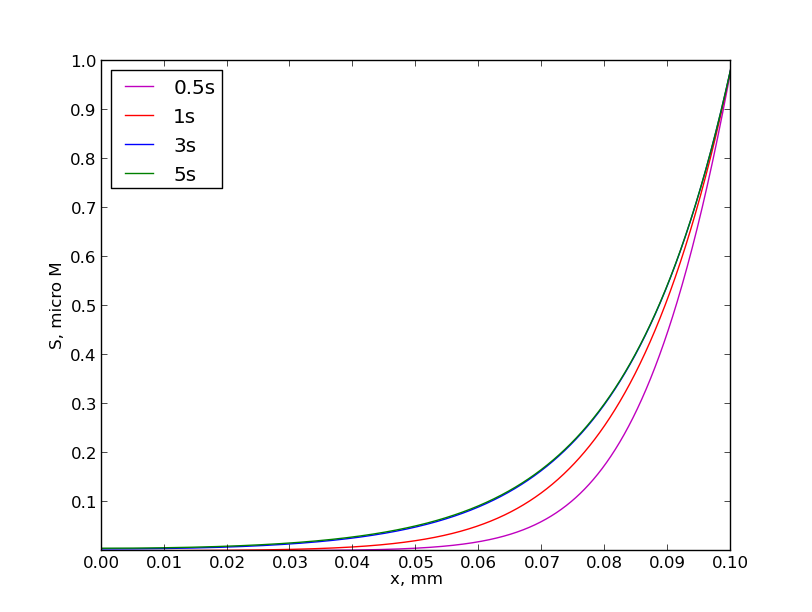
\includegraphics[scale=0.5]{img/S}
%     \caption{Substrate}
%     \label{img:mlp}
% \end{figure}
% 
% \begin{figure}[H]
%     \centering
%     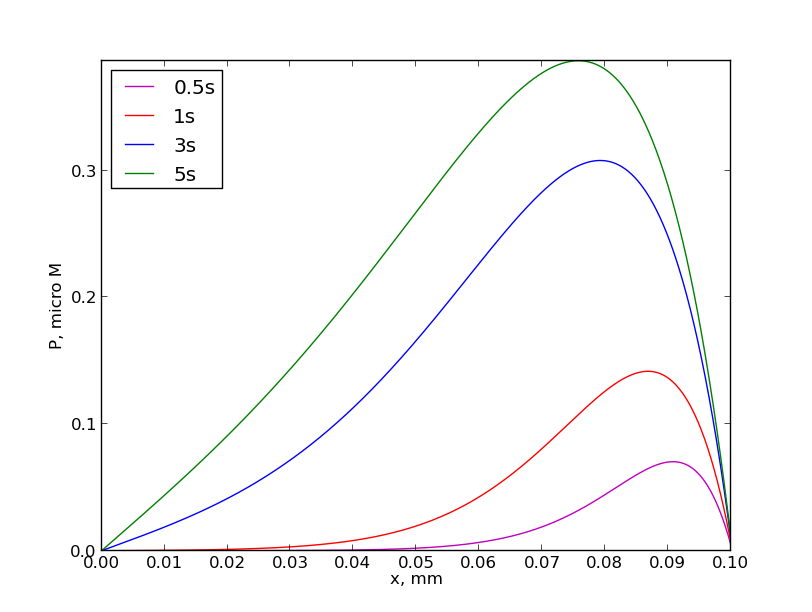
\includegraphics[scale=0.5]{img/P}
%     \caption{Product}
%     \label{img:mlp}
% \end{figure}
% 
% \begin{figure}[H]
%     \centering
%     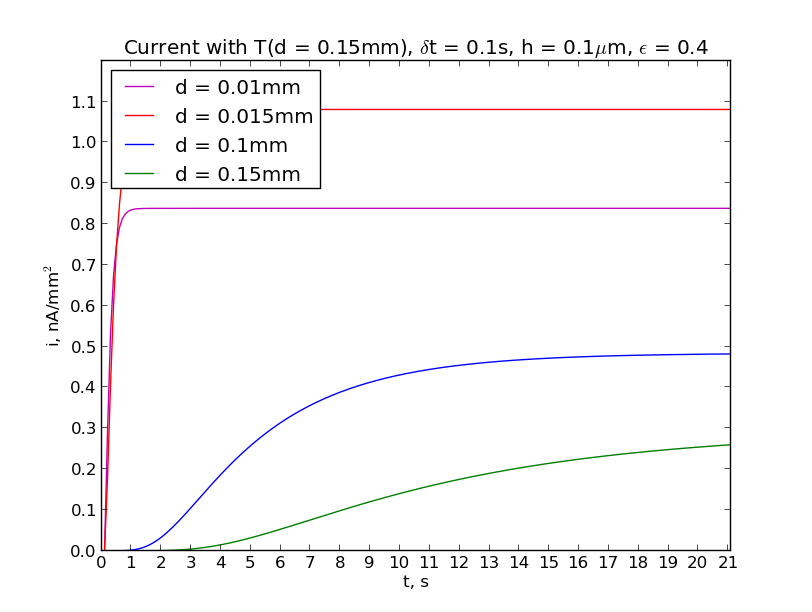
\includegraphics[scale=0.5]{img/i}
%     \caption{Current}
%     \label{img:mlp}
% \end{figure}
% 
%\appendix
%----------------------------------------------------

\bibliography{bibliografija}


%\appendix
%\section{Papildomų eksperimentų rezultatų lentelės}
%\begin{figure}[H]
%    \centering
%    \includegraphics[scale=0.5]{img/MLP}
%    \caption{Paveikslėlio pavyzdys}
%    \label{img:mlp}
%\end{figure}
%
\end{document}
